\documentclass[final]{beamer}\usepackage[]{graphicx}\usepackage[]{color}
%% maxwidth is the original width if it is less than linewidth
%% otherwise use linewidth (to make sure the graphics do not exceed the margin)
\makeatletter
\def\maxwidth{ %
  \ifdim\Gin@nat@width>\linewidth
    \linewidth
  \else
    \Gin@nat@width
  \fi
}
\makeatother

\definecolor{fgcolor}{rgb}{0.345, 0.345, 0.345}
\newcommand{\hlnum}[1]{\textcolor[rgb]{0.686,0.059,0.569}{#1}}%
\newcommand{\hlstr}[1]{\textcolor[rgb]{0.192,0.494,0.8}{#1}}%
\newcommand{\hlcom}[1]{\textcolor[rgb]{0.678,0.584,0.686}{\textit{#1}}}%
\newcommand{\hlopt}[1]{\textcolor[rgb]{0,0,0}{#1}}%
\newcommand{\hlstd}[1]{\textcolor[rgb]{0.345,0.345,0.345}{#1}}%
\newcommand{\hlkwa}[1]{\textcolor[rgb]{0.161,0.373,0.58}{\textbf{#1}}}%
\newcommand{\hlkwb}[1]{\textcolor[rgb]{0.69,0.353,0.396}{#1}}%
\newcommand{\hlkwc}[1]{\textcolor[rgb]{0.333,0.667,0.333}{#1}}%
\newcommand{\hlkwd}[1]{\textcolor[rgb]{0.737,0.353,0.396}{\textbf{#1}}}%
\let\hlipl\hlkwb

\usepackage{framed}
\makeatletter
\newenvironment{kframe}{%
 \def\at@end@of@kframe{}%
 \ifinner\ifhmode%
  \def\at@end@of@kframe{\end{minipage}}%
  \begin{minipage}{\columnwidth}%
 \fi\fi%
 \def\FrameCommand##1{\hskip\@totalleftmargin \hskip-\fboxsep
 \colorbox{shadecolor}{##1}\hskip-\fboxsep
     % There is no \\@totalrightmargin, so:
     \hskip-\linewidth \hskip-\@totalleftmargin \hskip\columnwidth}%
 \MakeFramed {\advance\hsize-\width
   \@totalleftmargin\z@ \linewidth\hsize
   \@setminipage}}%
 {\par\unskip\endMakeFramed%
 \at@end@of@kframe}
\makeatother

\definecolor{shadecolor}{rgb}{.97, .97, .97}
\definecolor{messagecolor}{rgb}{0, 0, 0}
\definecolor{warningcolor}{rgb}{1, 0, 1}
\definecolor{errorcolor}{rgb}{1, 0, 0}
\newenvironment{knitrout}{}{} % an empty environment to be redefined in TeX

\usepackage{alltt}

\mode<presentation>{\usetheme{confposter}}
\usepackage{amsmath, amsfonts, amssymb, pxfonts, eulervm, xspace, enumerate, hyperref, color, bookmark}
\usepackage{graphicx}
\usepackage[orientation=landscape, size=custom, width =152.4, height=106.68, scale=1.4, debug]{beamerposter}
\setbeamercolor{block title}{fg=black,bg=lyellow} % Colors of the block titles
\setbeamercolor{block body}{fg=black,bg=lyellow} % Colors of the body of blocks
\setbeamercolor{block alerted title}{fg=white,bg=black} % Colors of the highlighted block titles
\setbeamercolor{block alerted body}{fg=black,bg=white} % Colors of the body of highlighted blocks
% Many more colors are available for use in beamerthemeconfposter.sty

%-----------------------------------------------------------
% Define the column widths and overall poster size
% To set effective sepwid, onecolwid and twocolwid values, first choose how many columns you want and how much separation you want between columns
% In this template, the separation width chosen is 0.024 of the paper width and a 4-column layout
% onecolwid should therefore be (1-(# of columns+1)*sepwid)/# of columns e.g. (1-(4+1)*0.024)/4 = 0.22
% Set twocolwid to be (2*onecolwid)+sepwid = 0.464
% Set threecolwid to be (3*onecolwid)+2*sepwid = 0.708

\newlength{\sepwid}
\newlength{\onecolwid}
\newlength{\twocolwid}
\newlength{\threecolwid}
\setlength{\sepwid}{0.024\paperwidth} % Separation width (white space) between columns
\setlength{\onecolwid}{0.22\paperwidth} % Width of one column
\setlength{\twocolwid}{0.464\paperwidth} % Width of two columns
\setlength{\threecolwid}{0.708\paperwidth} % Width of three columns
\setlength{\topmargin}{-0.5in} % Reduce the top margin size
%-----------------------------------------------------------

\usepackage{graphicx}  % Required for including images

\usepackage{booktabs} % Top and bottom rules for tables

%----------------------------------------------------------------------------------------
%	TITLE SECTION 
%----------------------------------------------------------------------------------------

\def\conference{The Conference Name Here}
\title{Analyzing and Influencing Carbon Sequestration}
\author{Ben Jones, Hannah X Laws, Andrew Sullivan, Kelly Loucks} 
\institute{Department of Mathematical Sciences}

%----------------------------------------------------------------------------------------
\IfFileExists{upquote.sty}{\usepackage{upquote}}{}
\begin{document}

\addtobeamertemplate{block end}{}{\vspace*{2ex}} % White space under blocks
\addtobeamertemplate{block alerted end}{}{\vspace*{2ex}} % White space under highlighted (alert) blocks

\setlength{\belowcaptionskip}{2ex} % White space under figures
\setlength\belowdisplayshortskip{2ex} % White space under equations

\begin{frame}[t] % The whole poster is enclosed in one beamer frame

\begin{tikzpicture}[remember picture,overlay]
%add logos in corners
\node[anchor=north west] at ([shift={(3cm,0cm)}]current page.north west)
    {
\includegraphics[width=8cm]{usfs.png}};
\node[anchor=north east] at ([shift={(-3cm,-1cm)}]current page.north east)
    {
\includegraphics[width=22cm]{app.png}};
\end{tikzpicture}

\begin{columns}[t] % The whole poster consists of three major columns, the second of which is split into two columns twice - the [t] option aligns each column's content to the top

\begin{column}{\sepwid}\end{column} % Empty spacer column

\begin{column}{\onecolwid} % The first column

%----------------------------------------------------------------------------------------
%	Abstract
%----------------------------------------------------------------------------------------

\begin{alertblock}{Abstract}
Sequestration of carbon in forests is a process that can pull large quantities of carbon out of the atmosphere or prevent its release to the atmosphere, 87\% of total CO2 removals in 2014. Carbon mitigation efforts have thus focused much attention on reforestation, forest management,and forest based products. According to the most recent report to the UNFCCC, an estimated 18.7\% of the total carbon in woody materials is contained in harvested wood (HWP and SWDS).  


The amount of carbon in HWP and SWDS depend on how much wood is harvested, what types of products are produced, how the products are used, the lifetime of the wood products, and how the wood is processed at the end of its primary product lifetime.

\end{alertblock}

%----------------------------------------------------------------------------------------
%	INTRODUCTION
%----------------------------------------------------------------------------------------

\begin{block}{Carbon Contributions}
\begin{itemize}
\item In 2005, the contribution to removals was 30 Tg (million metric tons) C (carbon) and 31 Tg C for the Production and Atmospheric Flow Approaches, respectively, and 44 Tg C for the Stock Change Approach. This range is 17 to 25 percent of C removals by forests, or would offset 42 percent to 61 percent of residential natural gas C emissions in 2005. 
\vspace{1ex}
\item The contribution has declined under the Production and Atmospheric Flow Approaches since 1990 and has increased under the Stock Change Approach. The Stock Change estimate has increased because it explicitly includes C in increasing net imports of wood and paper products. 
\vspace{1ex}
\end{itemize}
\vspace{0ex}
\vfill
\end{block}

%------------------------------------------------

%-- Block 1-3
\begin{block}{Sources of Data and Equations}

\begin{enumerate}[I.]
\item WOODCARB II Software in Microsoft Excel\textsuperscript{\textregistered}
\vspace{0ex}
Note: Base level data was given in spreadsheet. 
\item Harvest Quantities:
\item Imports, Exports, etc.:
\item Decay of HWP:
\end{enumerate}
\vspace{0ex}

\end{block}
\vfill

%-- Block 1-4

\begin{block}{Accounting Approaches}

\begin{itemize}
\item International workshops identified three approaches to re- port HWP contribution. These approaches focus on account- ing differently for changes in carbon in HWP imports and exports.
\item Stock Change:
\item Production:
\item Atmospheric Flow:
\end{itemize}


\end{block}
\vfill

%-- Block 1-5

\begin{block}{Access to Packages}

\begin{enumerate}
\item Our incredible \href{http://madeitup.com}{web page}
\item Our incredible \href{http://benjones2.github.io/WOODCARB3R/}{WOODCARB3R package}
\end{enumerate}


\end{block}
\vfill

%----------------------------------------------------------------------------------------

\end{column} % End of the first column

\begin{column}{\sepwid}\end{column} % Empty spacer column

\begin{column}{\twocolwid} % Begin a column which is two columns wide (column 2)

\begin{columns}[t,totalwidth=\twocolwid] % Split up the two columns wide column

\begin{column}{\onecolwid}\vspace{-.6in} % The first column within column 2 (column 2.1)

%----------------------------------------------------------------------------------------
%	PURPOSE
%----------------------------------------------------------------------------------------

\begin{block}{Purpose}
\vspace{0ex}
\begin{itemize}
\item Information is intended to aid in international discussions and any agreements about managing greenhouse gas emissions and sinks.
\item Also provides national level methods and estimates of carbon sinks and emissions associated with HWP.
\item
\end{itemize}
\vspace{-1.5ex}
\end{block}

%----------------------------------------------------------------------------------------

\end{column} % End of column 2.1

\begin{column}{\onecolwid}\vspace{-.6in} % The second column within column 2 (column 2.2)

%----------------------------------------------------------------------------------------
%	Current Analysis
%----------------------------------------------------------------------------------------

\begin{block}{Current Analysis}
\vspace{0ex}
\begin{itemize}
\item The contribution estimates were validated by adjusting the half-life of products in use in order to match independent estimates of carbon in housing in 2001 and annual wood and paper discards to solid-waste disposal sites (SWDS) during 1990 to 2001. 
\item
\item
\item
\end{itemize}
\end{block}

%----------------------------------------------------------------------------------------

\end{column} % End of column 2.2

\end{columns} % End of the split of column 2 - any content after this will now take up 2 columns width

%----------------------------------------------------------------------------------------
%	GRAPH
%----------------------------------------------------------------------------------------

\begin{alertblock}{Total Carbon Removals}
\vspace{0ex}
\centering
\begin{knitrout}
\definecolor{shadecolor}{rgb}{0.969, 0.969, 0.969}\color{fgcolor}

{\centering 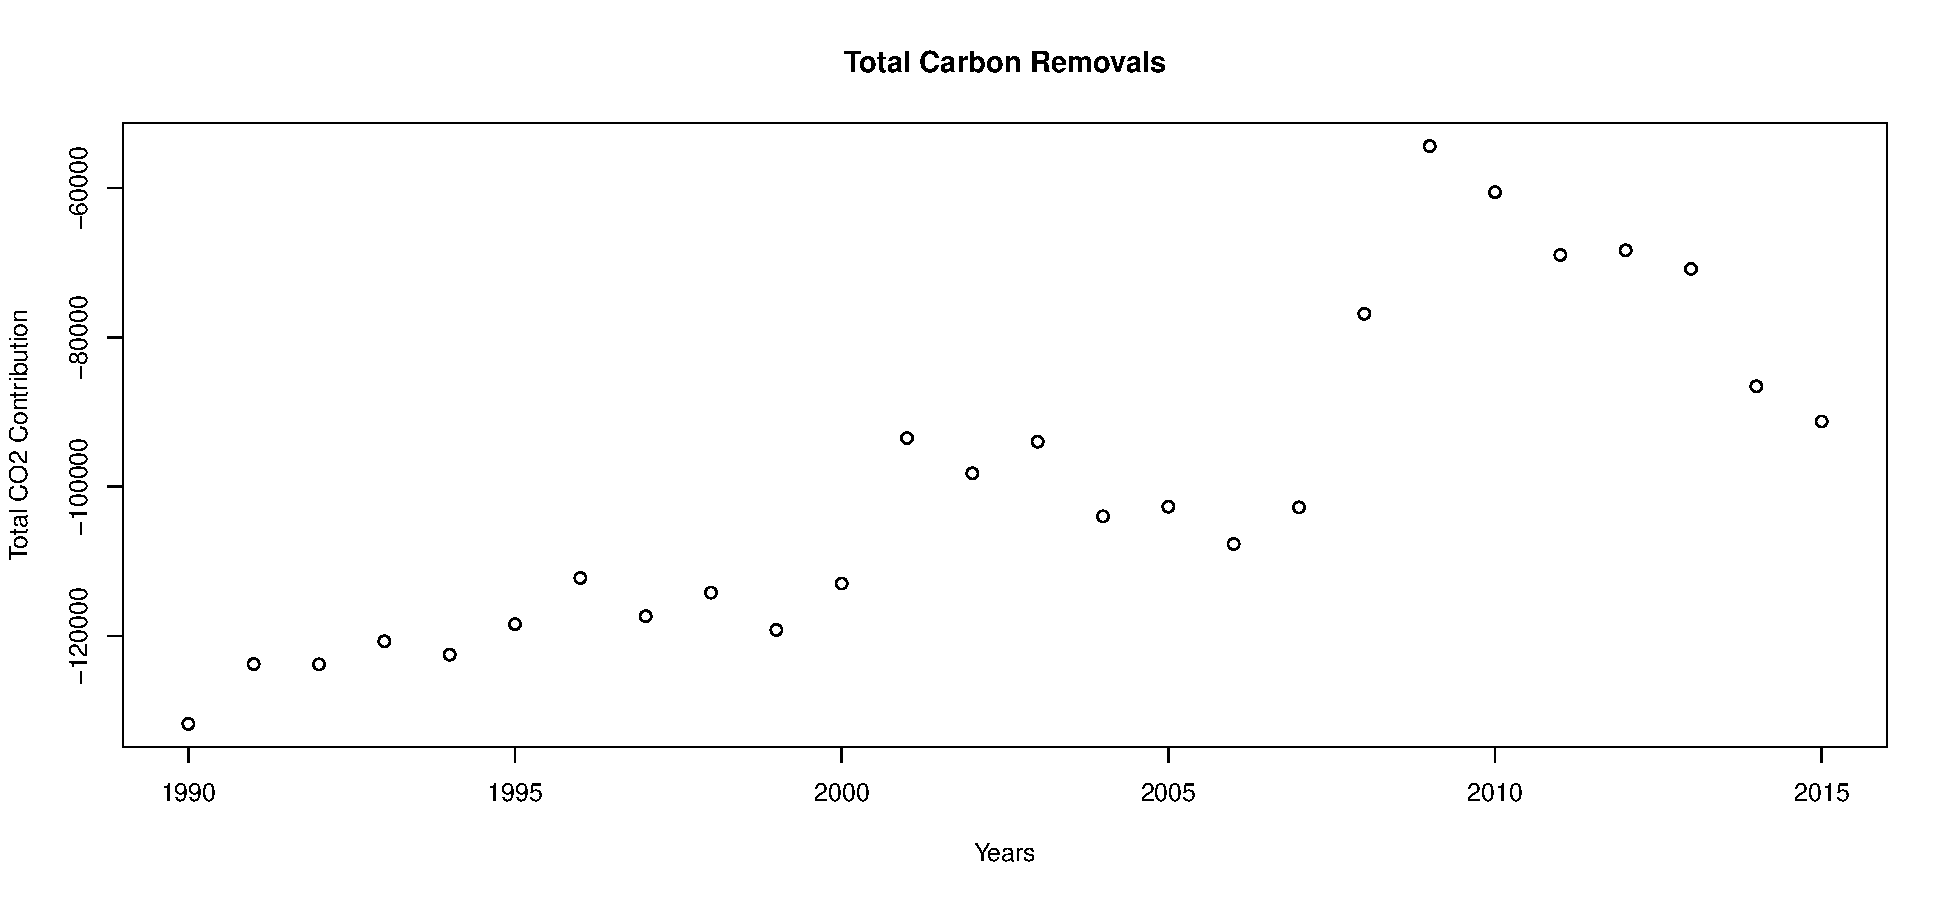
\includegraphics[width=\maxwidth]{figure/RCODE-1} 

}



\end{knitrout}
\vfill
\end{alertblock} 

%----------------------------------------------------------------------------------------

\begin{columns}[t,totalwidth=\twocolwid] % Split up the two columns wide column again

\begin{column}{\onecolwid} % The first column within column 2 (column 2.1)

%----------------------------------------------------------------------------------------
%	Sensitivity Analysis
%----------------------------------------------------------------------------------------

\begin{block}{Sensitvity Analysis}
\begin{itemize}
\item Used to determine how different values of an independent variable impact a particular dependent variable under a given set of assumptions. 
\item How the uncertainty in the output of a mathematical model or system can be apportioned to different sources of uncertainty in its inputs.
\item Helps in identifying the key variables that are major influence in the cost and benefits of the project.
\item 
\end{itemize}

\end{block}

%----------------------------------------------------------------------------------------

\end{column} % End of column 2.1

\begin{column}{\onecolwid} % The second column within column 2 (column 2.2)

%----------------------------------------------------------------------------------------
%	Methods for Analyzing Sensitivity
%----------------------------------------------------------------------------------------

\begin{block}{Methods for Analyzing Sensitivity}
\begin{itemize}
\item A Monte-Carlo simulation used to assess the effect of uncertainty in inputs suggests the 90 percent confidence interval for removal contribution estimates under the three approaches is within –23\% to +19\%.
\vspace{2ex}
\item Monte Carlo simulation is a computerized mathematical technique that allows people to account for risk in quantitative analysis and decision making.
\item
\item
\end{itemize}
\end{block}

%----------------------------------------------------------------------------------------

\end{column} % End of column 2.2

\end{columns} % End of the split of column 2

\end{column} % End of the second column

\begin{column}{\sepwid}\end{column} % Empty spacer column

\begin{column}{\onecolwid} % The third column

%----------------------------------------------------------------------------------------
%	POTENTIAL STRATEGIES
%----------------------------------------------------------------------------------------

\begin{block}{Potential Strategies}
\vspace{0ex}
\begin{itemize}
\item
\item
\item
\item
\end{itemize}
\vspace{0ex}
\vfill
\end{block}
\vfill

%----------------------------------------------------------------------------------------
% CONCLUSIONS
%----------------------------------------------------------------------------------------

\begin{block}{Conclusions}
\begin{itemize}
\item
\item
\item
\end{itemize}
\vspace{0ex}
\vfill
\end{block}
\vfill
%--------------------------------------------------------
% POSSIBLE EXTENSIONS
%--------------------------------------------------------
\begin{block}{Possible Extensions}
\begin{itemize}
\item  
\item  
\item  
\end{itemize}
\vspace{0ex}
\vfill
\end{block}
\vfill

%----------------------------------------------------------------------------------------
%	REFERENCES
%----------------------------------------------------------------------------------------
\begin{block}{References}
\footnotesize
\setbeamertemplate{bibliography item}[text]
\vspace{-1ex}


\bibliographystyle{plain}  % can use plain but comment out natbib at top if using plain
\bibliography{knitr-packages,poster}
\normalsize
\vfill
\end{block} 
\vfill


%----------------------------------------------------------------------------------------
%	ACKNOWLEDGEMENTS
%----------------------------------------------------------------------------------------

\setbeamercolor{block title}{fg=black,bg=white} % Change the block title color

\begin{block}{Acknowledgements}

\small{\rmfamily{.}} \\

\end{block}


\end{column} % End of the third column

\end{columns} % End of all the columns in the poster

\end{frame} % End of the enclosing frame

\end{document}


